%%%LaTeX文档的基本结构,编译和调试,命令符合的输入(如:%,$,{ ... },\)
%\documentclass[11pt]{article} 
\documentclass{book} %book,article,report,letter
\usepackage{amsmath} %宏包
\usepackage{float}
\usepackage{indentfirst}
\usepackage{lipsum}
\usepackage[english]{babel}
\usepackage{fontspec}
\newcommand{\tnewroman}{\fontspec{Times New Roman}}
\setmainfont{Times New Roman}%fontspec

\usepackage{amsmath,amssymb,amsthm}
\usepackage{graphicx}
\usepackage[margin=1in]{geometry}
\usepackage{fancyhdr}
\setlength{\parindent}{0pt}
\setlength{\parskip}{5pt plus 1pt}
\setlength{\headheight}{13.6pt}
\newcommand\question[2]{\vspace{.25in}\hrule\textbf{#1: #2}\vspace{.5em}\hrule\vspace{.10in}}
\renewcommand\part[1]{\vspace{.10in}\textbf{(#1)}}
\newcommand\algorithm{\vspace{.10in}\textbf{Algorithm: }}
\newcommand\correctness{\vspace{.10in}\textbf{Correctness: }}
\newcommand\runtime{\vspace{.10in}\textbf{Running time: }}
\pagestyle{fancyplain}
%\lhead{\textbf{\NAME\ (\ANDREWID)}}
\lhead{\textbf{SAR}}
%\chead{\textbf{HW\HWNUM}}
\rhead{ \today}
%导言区
\begin{document}
 
\title{Report of Operational Statistics for SAR }  %%书名
\author{Xiaoming Jiang: ID 19171213764} %%作者
%\date{} %%如果没有这句,会生成时间
\maketitle  %%生成书名
\newcommand\NAME{Carl Kingsford}  % your name
\newcommand\ANDREWID{ckingsf}     % your andrew id
\newcommand\HWNUM{}
\section{Exponential Distribution}
\setlength{\parindent}{2em}
The probability density function  of an exponential distribution is:
\begin{center}
	\begin{equation}
	f(x;\lambda)=
	\begin{cases}
	\lambda e^{-\lambda x}& \text{$x\geq $0}\\
	0& \text{$x < $0}
	\end{cases}
	\end{equation} 
\end{center}
The exponential density is showed in Figure1. 

\begin{figure}[H]
	\centering
	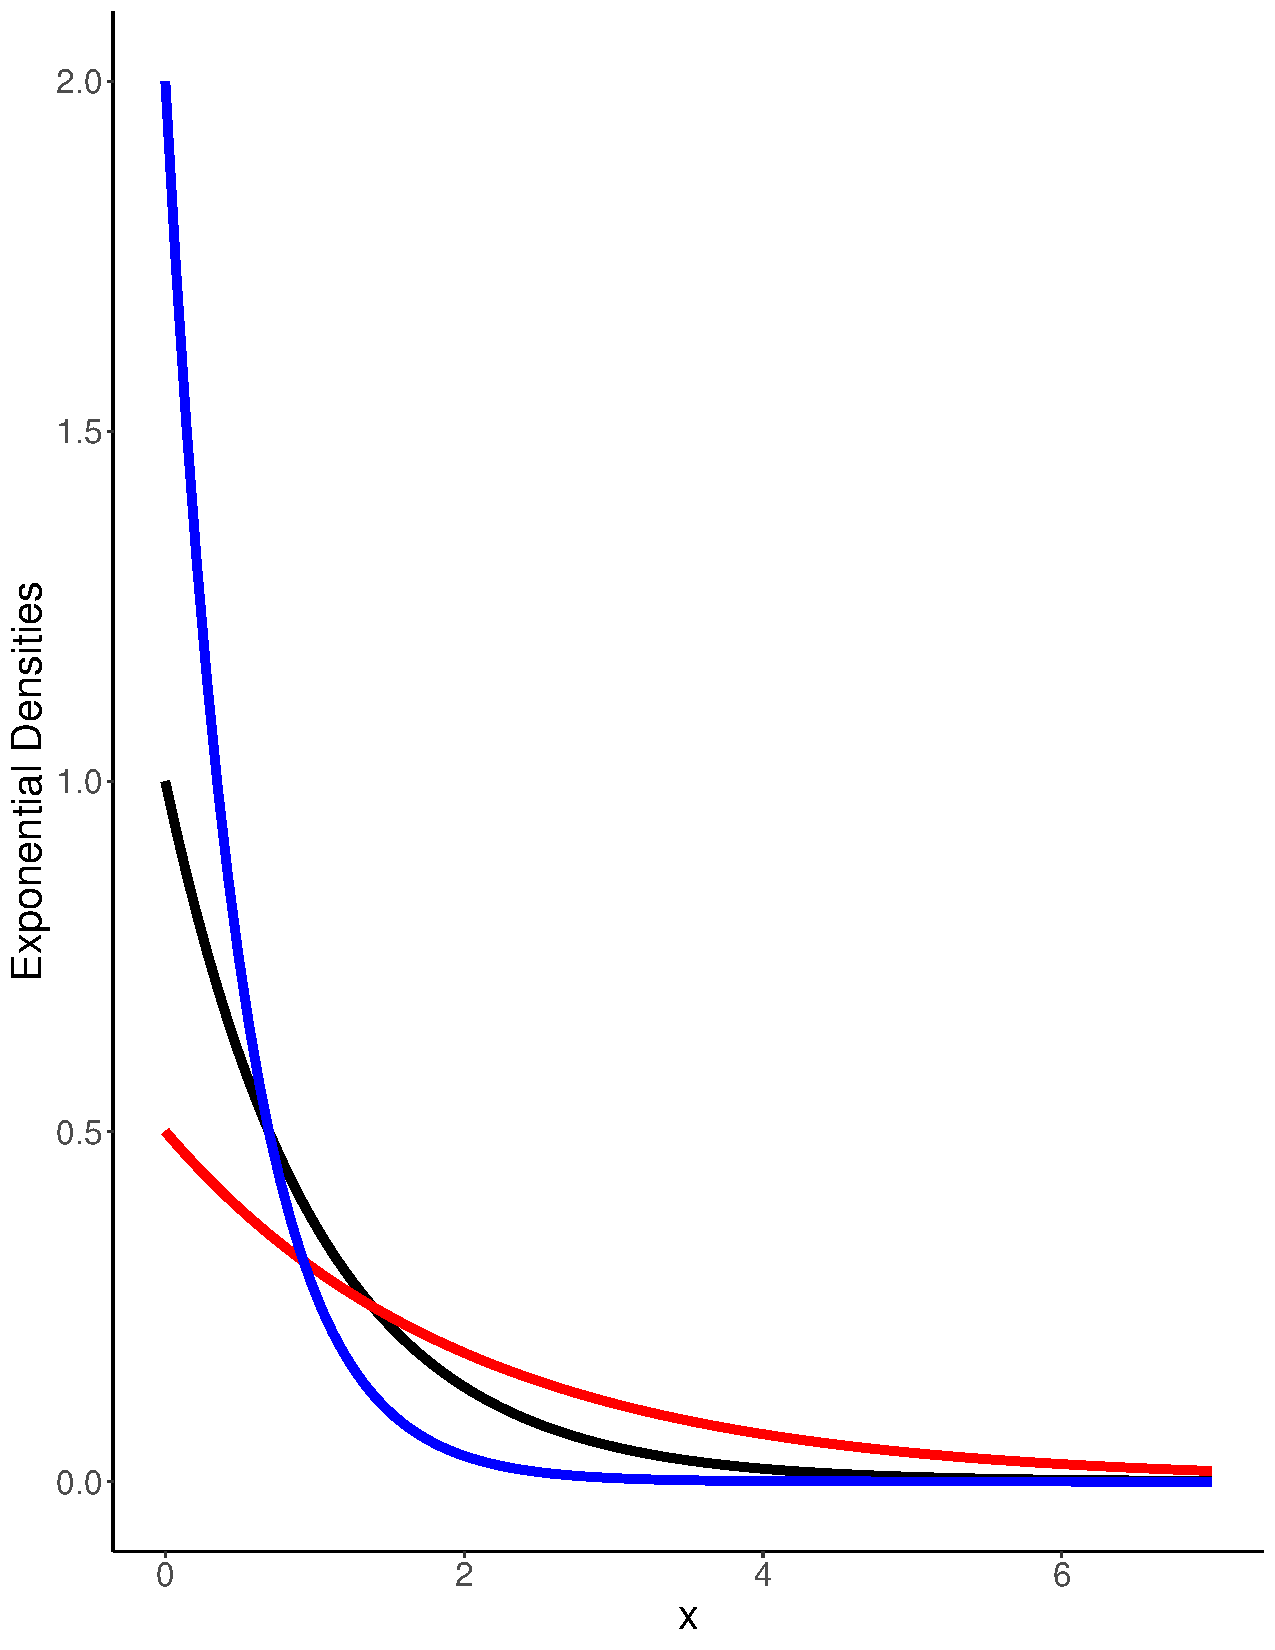
\includegraphics[width=0.7\linewidth,
	height=0.4\textheight]{exp_densities}
	\caption{}
	\label{fig:expdensities}
\end{figure}
\noindent The R code :\\
------------------------------------------------------------------------------------------\\
ggplot(data=data.frame(x=c(0, 7)), aes(x=x)) + \\
stat\_function(fun=dexp, geom = "line", size=2,col="black", args = (mean=1)) +\\
stat\_function(fun=dexp, geom = "line", size=2, col="red", args = (mean=.5)) +\\
stat\_function(fun=dexp, geom = "line", size=2, col="blue", args = (mean=2)) +\\
theme\_classic() +\\
theme(text = element\_text(size=20)) +\\
xlab("x") + ylab("Exponential Densities")\\
------------------------------------------------------------------------------------------\\
The cumulative distribution function is given by:\\
\begin{center}
	\begin{equation}
	F(x;\lambda)=
	\begin{cases}
	1- e^{-\lambda x}& \text{$x\geq $0}\\
	0& \text{$x < $0}
	\end{cases}
	\end{equation} 
\end{center}
The exponential distribution is showed in Figure2.
\begin{figure}[H]
	\centering
	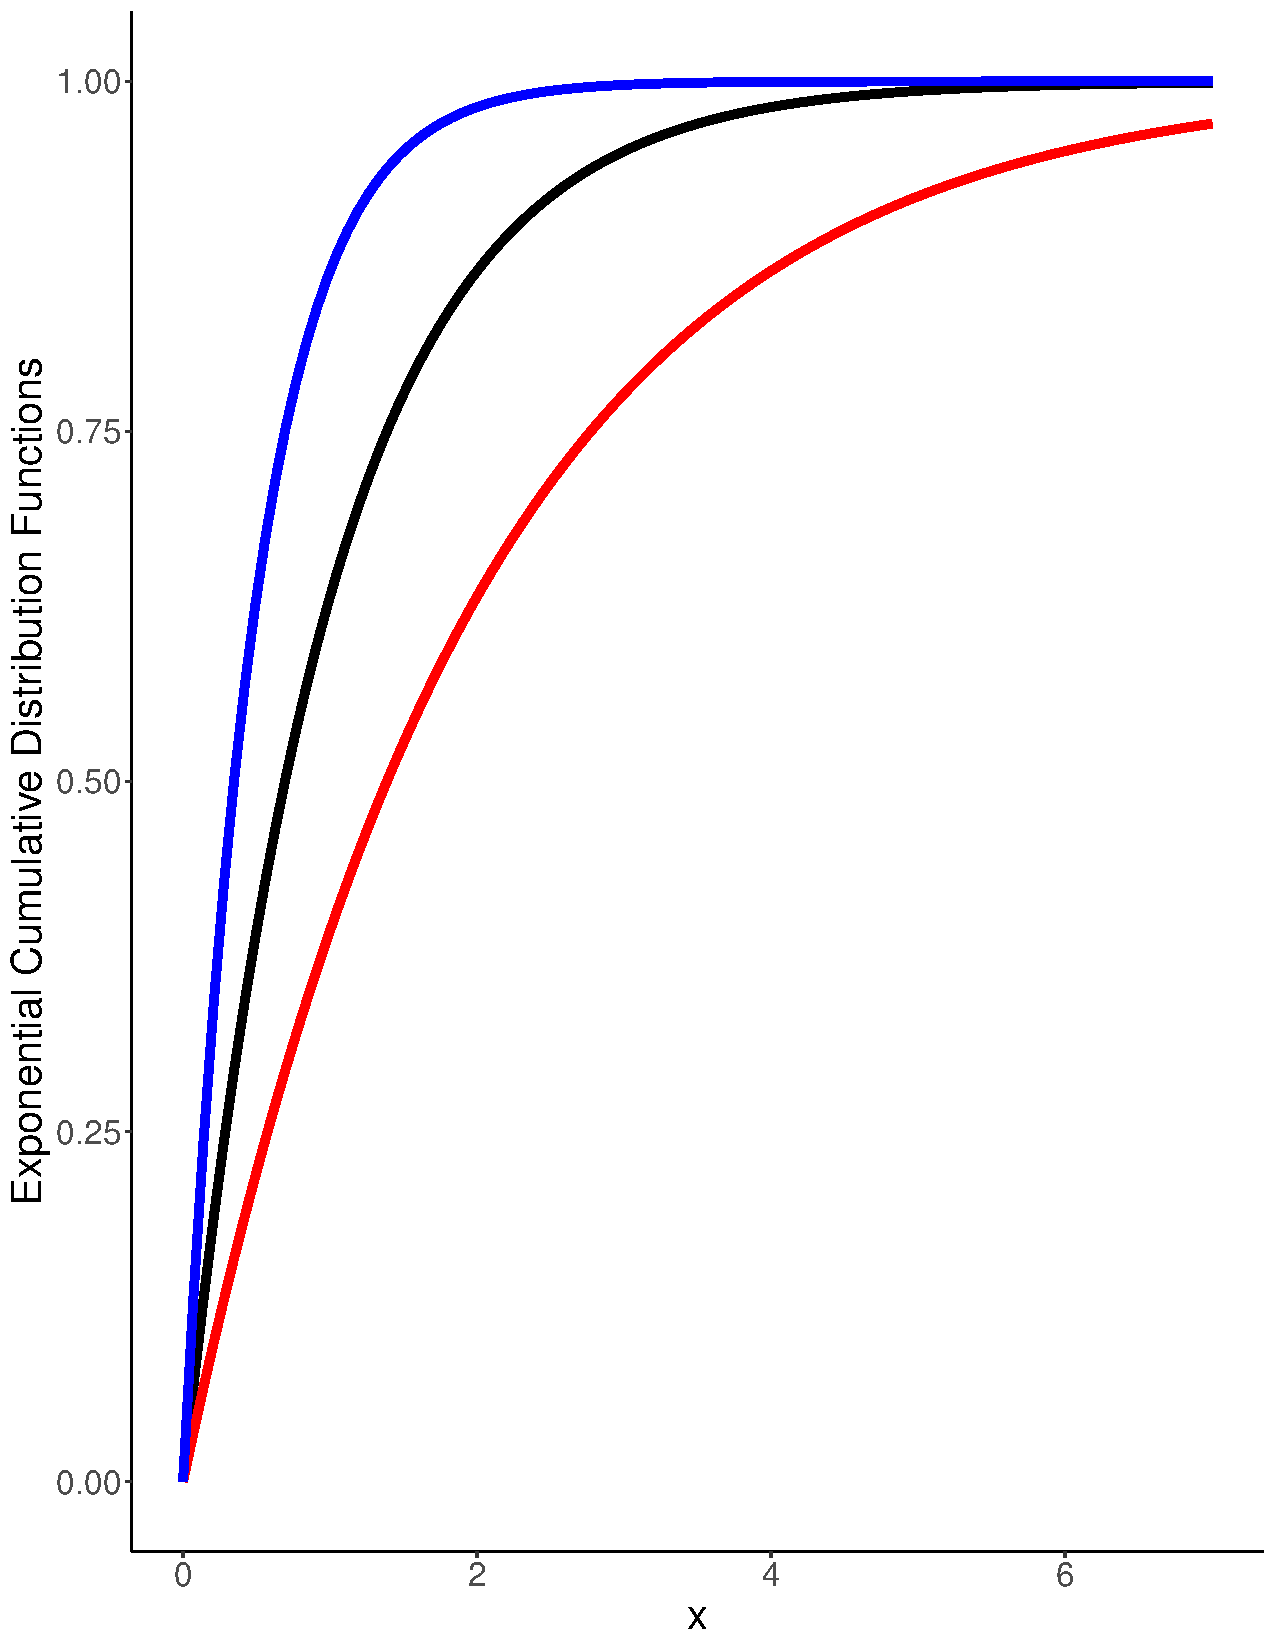
\includegraphics[width=0.7\linewidth, height=0.5\textheight]{dexp}
	\caption{}
	\label{fig:dexp}
\end{figure}
\noindent The R code :\\
------------------------------------------------------------------------------------------\\
ggplot(data=data.frame(x=seq(0, 7, length.out = 500)), aes(x=x)) +\\
stat\_function(fun=pexp, geom = "line", size=2, col="black", args = (mean=1)) +\\
stat\_function(fun=pexp, geom = "line", size=2, col="red", args = (mean=.5)) +\\
stat\_function(fun=pexp, geom = "line", size=2, col="blue", args = (mean=2)) +\\
theme\_classic() +\\
theme(text = element\_text(size=20)) +\\
xlab("x") + ylab("Exponential Cumulative Distribution Functions")\\
------------------------------------------------------------------------------------------\\
\section{Gamma Distribution}
The gamma distribution can be parameterized in terms of a shape parameter α = k and an inverse scale parameter β = 1/θ, called a rate parameter. A random variable X that is gamma-distributed with shape α and rate β is denoted.\\
\begin{center}
	\begin{equation}
	X\sim \Gamma (\alpha,\beta)\equiv Gamma(\alpha,\beta)
	\end{equation} 
\end{center}

The corresponding probability density function in the shape-rate parametrization is:
\begin{center}
	\begin{equation}
f(x;\alpha,\beta)=
\frac{\beta^\alpha x^{(\alpha-1)}e^{-\beta x}}{\Gamma(\alpha)}   
\qquad for \quad x >0 \quad a,p>0
\end{equation} 
\end{center}
The gamma density is showed in Figure3.
\begin{figure}[H]
	\centering
	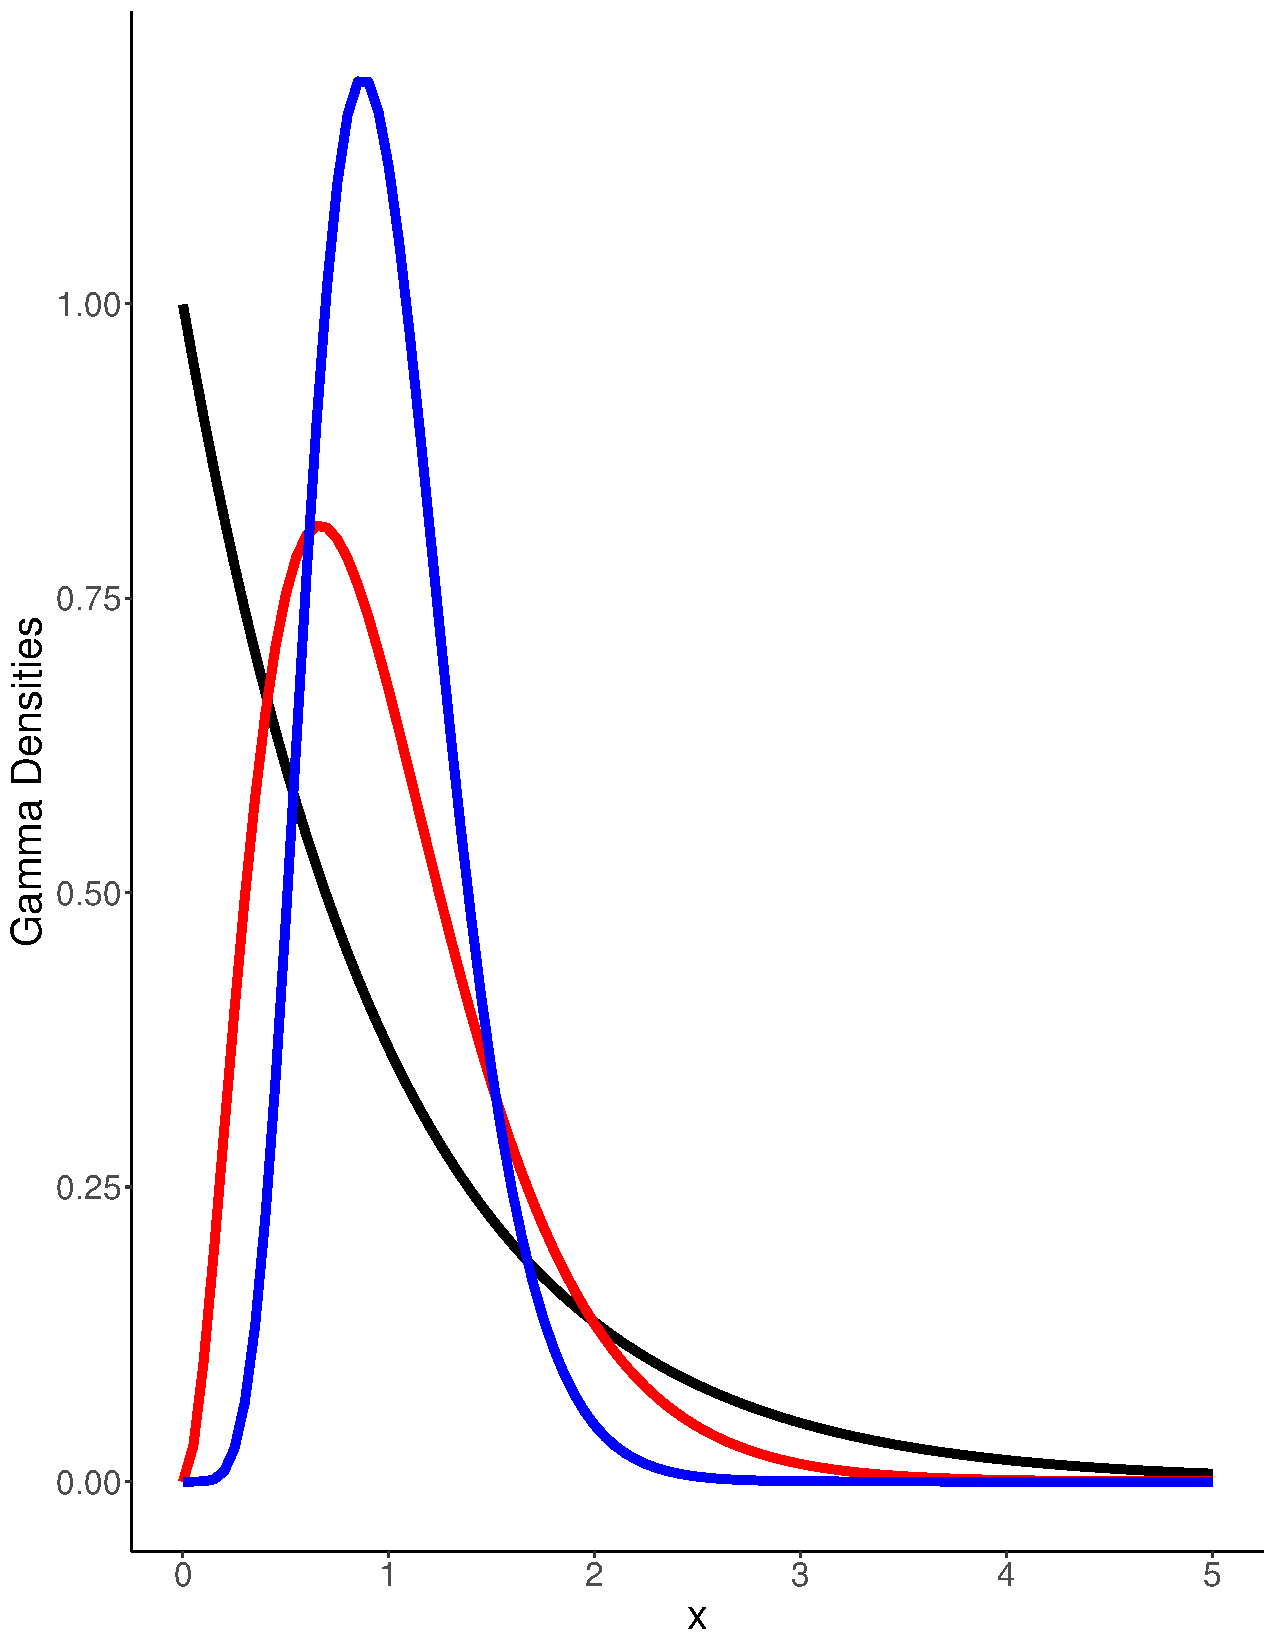
\includegraphics[width=0.7\linewidth,height=0.5\textheight]{gma_den}
	\caption{}
	\label{fig:gmaden}
\end{figure}
\noindent The R code :\\
------------------------------------------------------------------------------------------\\
ggplot(data=data.frame(x=seq(0.003,5,length.out = 500)), aes(x=x)) +\\
stat\_function(fun=dgamma, geom = "line", size=2, col="black", args = list(shape=1, scale=1)) +\\
stat\_function(fun=dgamma, geom = "line", size=2, col="red", args = list(shape=3, scale=1/3)) +\\
stat\_function(fun=dgamma, geom = "line", size=2, col="blue", args = list(shape=8,\\ scale=1/8)) +\\
theme\_classic() +\\
theme(text = element\_text(size=20)) +\\
xlab("x") + ylab("Gamma Densities")\\
------------------------------------------------------------------------------------------\\
The cumulative distribution function is the regularized gamma function:
\begin{center}
	\begin{equation}
	F(x;\alpha,\beta)=\int^a _b f(u;\alpha,\beta)du=\frac{\gamma(\alpha,\beta x)}{\Gamma(\alpha)}
	\end{equation} 
\end{center}
\noindent where $\displaystyle$ $\gamma$ ($\alpha$ ,$\beta$ x)$\displaystyle$ $\gamma$ ($\alpha$ ,$\beta$ x) is the lower incomplete gamma function.\\
\noindent If $\alpha$ is a positive integer , the cumulative distribution function has the following series expansion.
\begin{center}
	\begin{equation}
	F(x;\alpha,\beta)=1-\sum^{\alpha-1}_{i=1}\frac{(\beta x)^{i}}{i!}e^{-\beta x}=e^{-\beta x}\sum^{\infty}_{i=1}\frac{(\beta x)^{i}}{i!}
	\end{equation} 
\end{center}
The gamma distribution is showed in Figure4.
\begin{figure}[H]
	\centering
	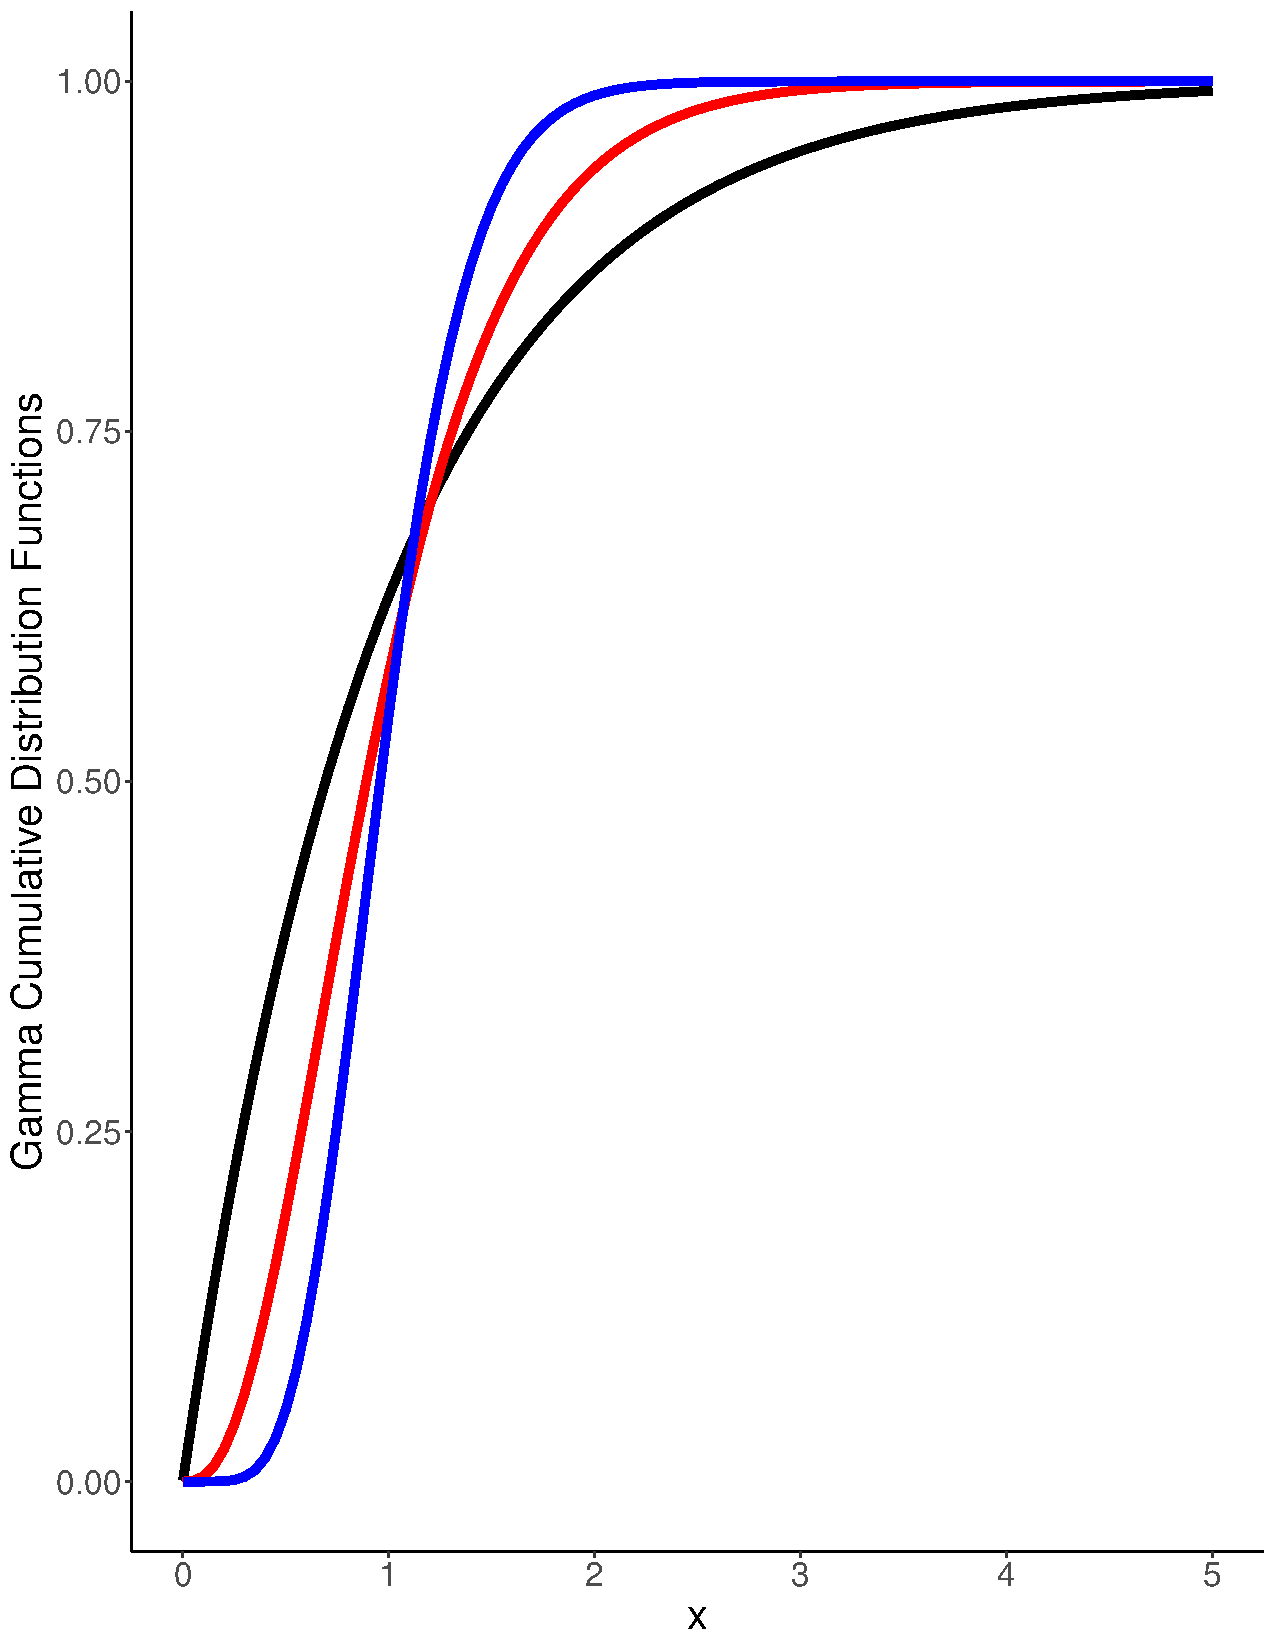
\includegraphics[width=0.7\linewidth,height=0.5\textheight]{dgamma_distri}
	\caption{}
	\label{fig:dgammadistri}
\end{figure}

\noindent The R code :\\
------------------------------------------------------------------------------------------\\
ggplot(data=data.frame(x=seq(0.003, 5, length.out = 500)), aes(x=x)) +\\
stat\_function(fun=pgamma, geom = "line", size=2, col="black", args = list(shape=1, scale=1)) +\\
stat\_function(fun=pgamma, geom = "line", size=2, col="red", args = list(shape=3, scale=1/3)) +\\
stat\_function(fun=pgamma, geom = "line", size=2, col="blue", args = list(shape=8, scale=1/8)) +\\
theme\_classic() +\\
theme(text = element\_text(size=20)) +\\
xlab("x") + ylab("Gamma Cumulative Distribution Functions")\\
------------------------------------------------------------------------------------------\\
\section{Beta distribution}
The probability density function of the beta distribution, for 0 ≤ x ≤ 1, and shape parameters α, β > 0, is a power function of the variable x and of its reflection (1 − x) as follows:

\begin{center}
\begin{equation}
f(x;\alpha,\beta)=\frac{1}{B(\alpha,\beta)}x^{(\alpha-1)}(1-x)^{(\beta-1)}
\end{equation} 
\end{center}
The beta density is showed in Figure4.
\begin{figure}[H]
	\centering
	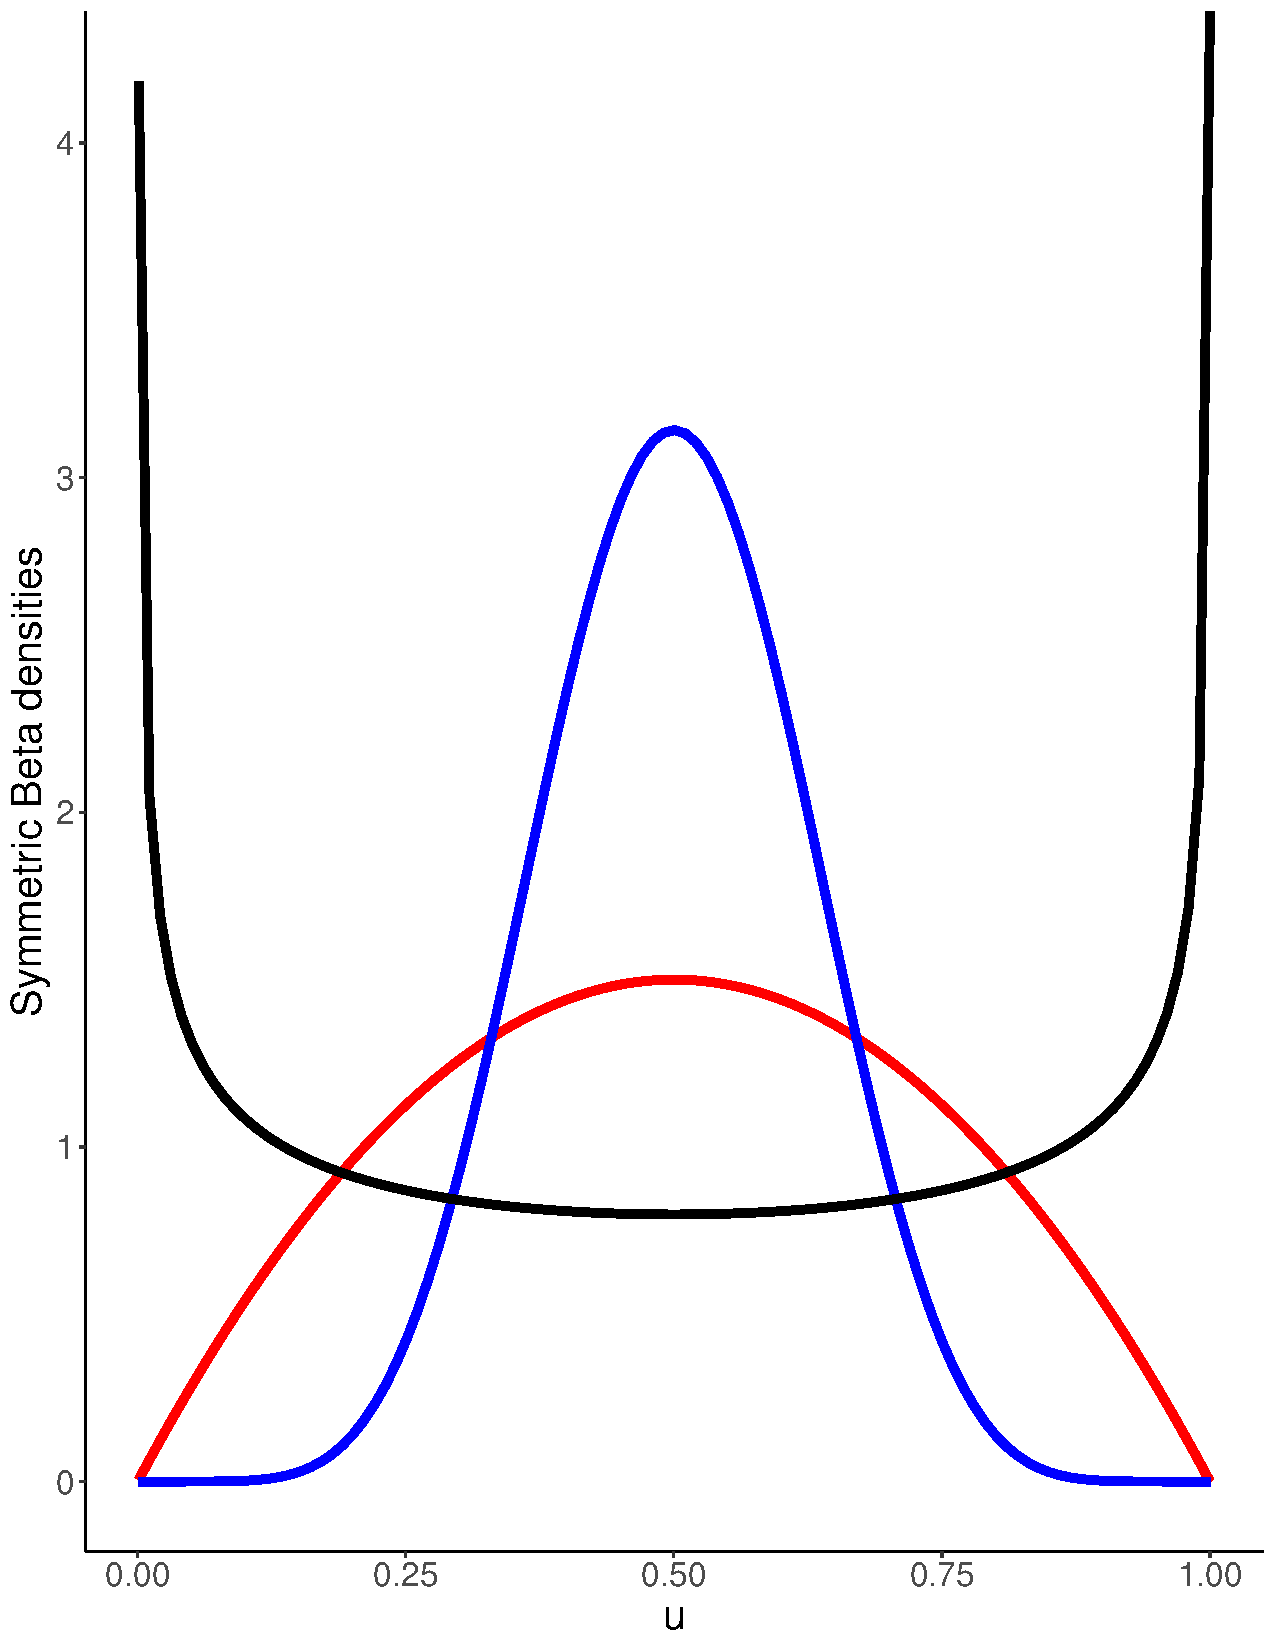
\includegraphics[width=0.7\linewidth,height=0.5\textheight]{beta}
	\caption{}
	\label{fig:beta}
\end{figure}

\noindent The R code :\\
------------------------------------------------------------------------------------------\\
ggplot(data=data.frame(x=seq(0.001, 1, length.out = 500)), aes(x=x)) +\\
stat\_function(fun=dbeta, geom = "line", size=2, col="red", args = list(shape1=2, shape2=2)) +\\
stat\_function(fun=dbeta, geom = "line", size=2, col="blue", args = list(shape1=8, shape2=8)) +\\
stat\_function(fun=dbeta, geom = "line", size=2, col="black", args = list(shape1=.7, shape2=.7)) +\\
theme\_classic() +\\
theme(text = element\_text(size=20)) +\\
xlab("u") + ylab("Symmetric Beta densities")\\
------------------------------------------------------------------------------------------\\
\section{Experiment}
I select  a part of the forest as followed:
\begin{figure}[H]
	\centering
	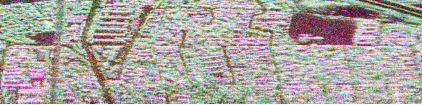
\includegraphics[width=0.7\linewidth]{sar_home_work2}
	\caption{}
	\label{fig:sarhomework2}
\end{figure}
Firstly,I convert the RGB image to a gray image.
\begin{figure}[H]
	\centering
	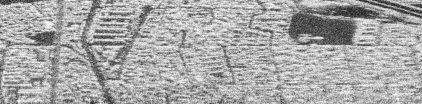
\includegraphics[width=0.7\linewidth]{sar_home_work1}
	\caption{}
	\label{fig:sarhomework1}
\end{figure}
then, loading the gray image and normalize the gray value.I use the hist function to produce the histogram as Figure8.
\begin{figure}[H]
	\centering
	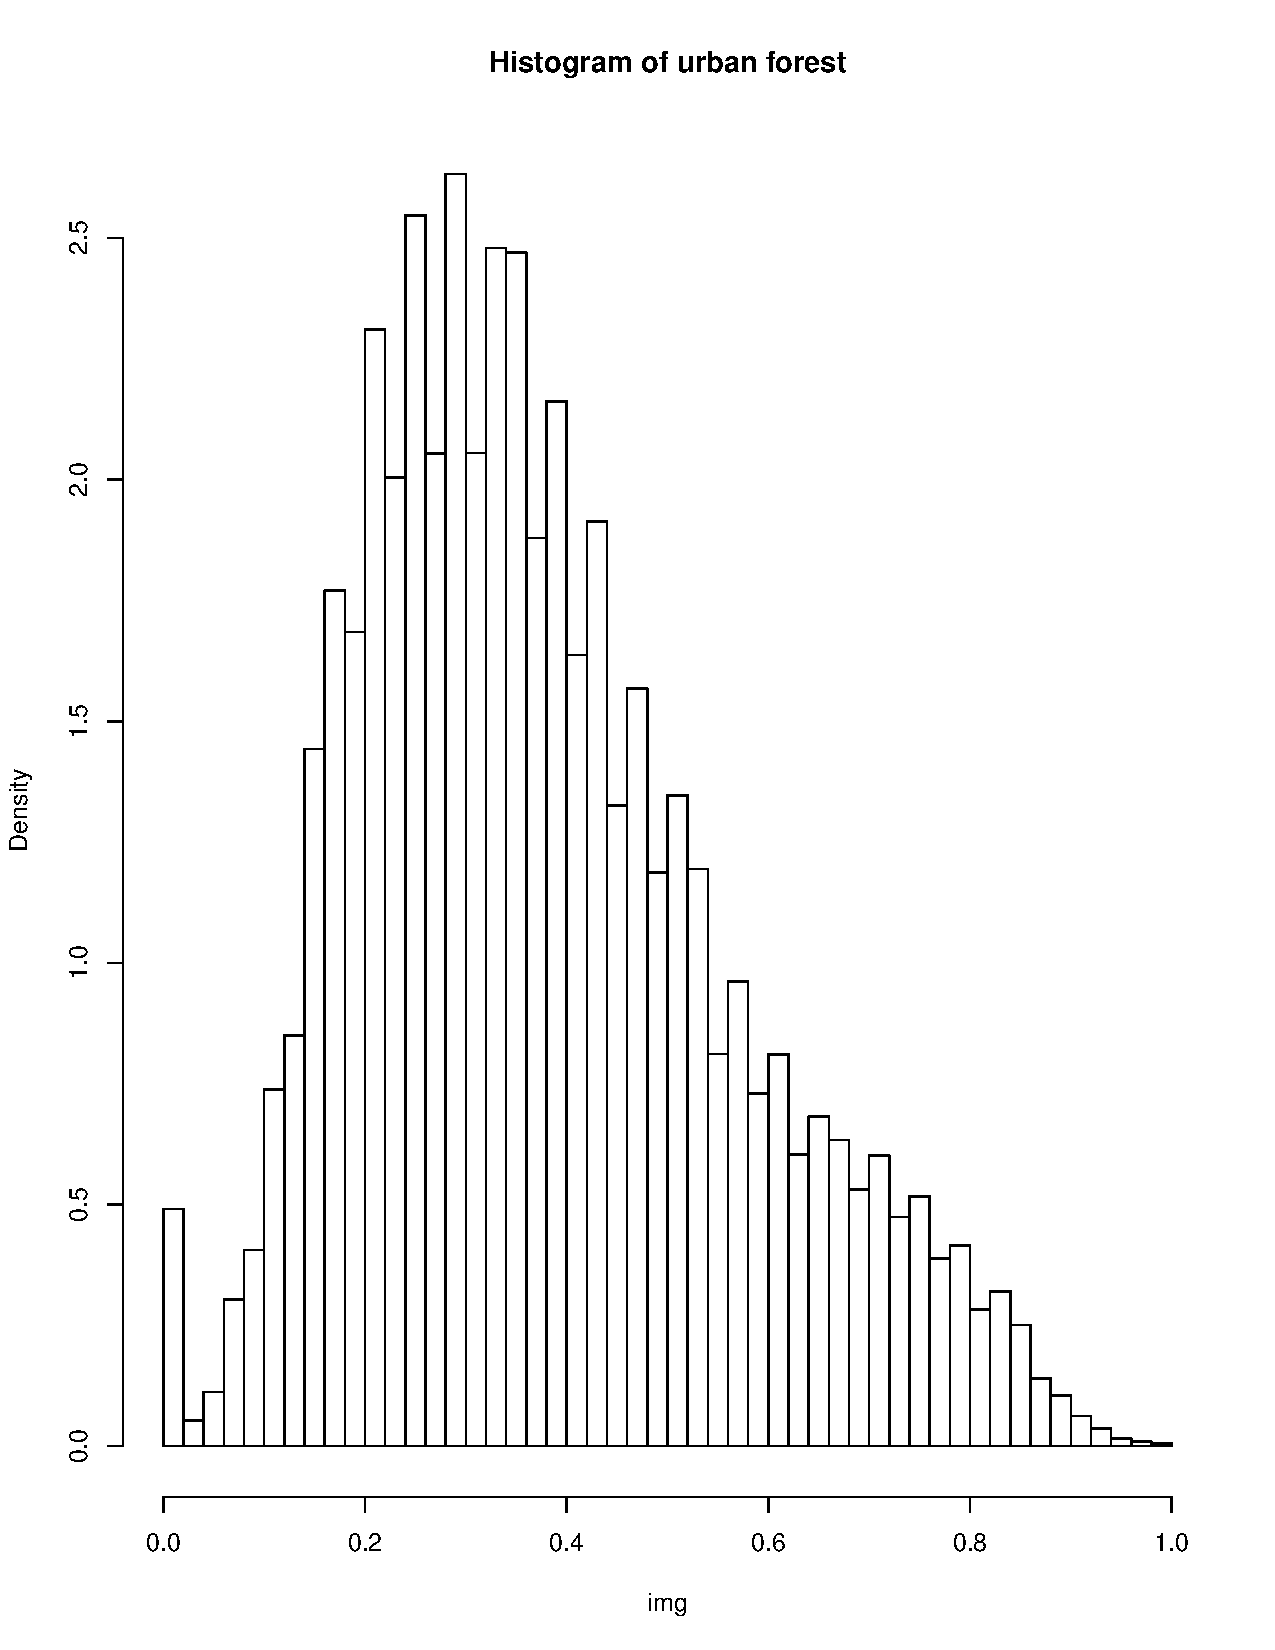
\includegraphics[width=0.7\linewidth,height=0.4\textheight]{Rplot01}
	\caption{}
	\label{fig:rplot01}
\end{figure}
Finally,i use ggplot function to produce Figure9. At the same time, gamma function  fitting is better when shape=4,scale=1/10.
\begin{figure}[H]
	\centering
	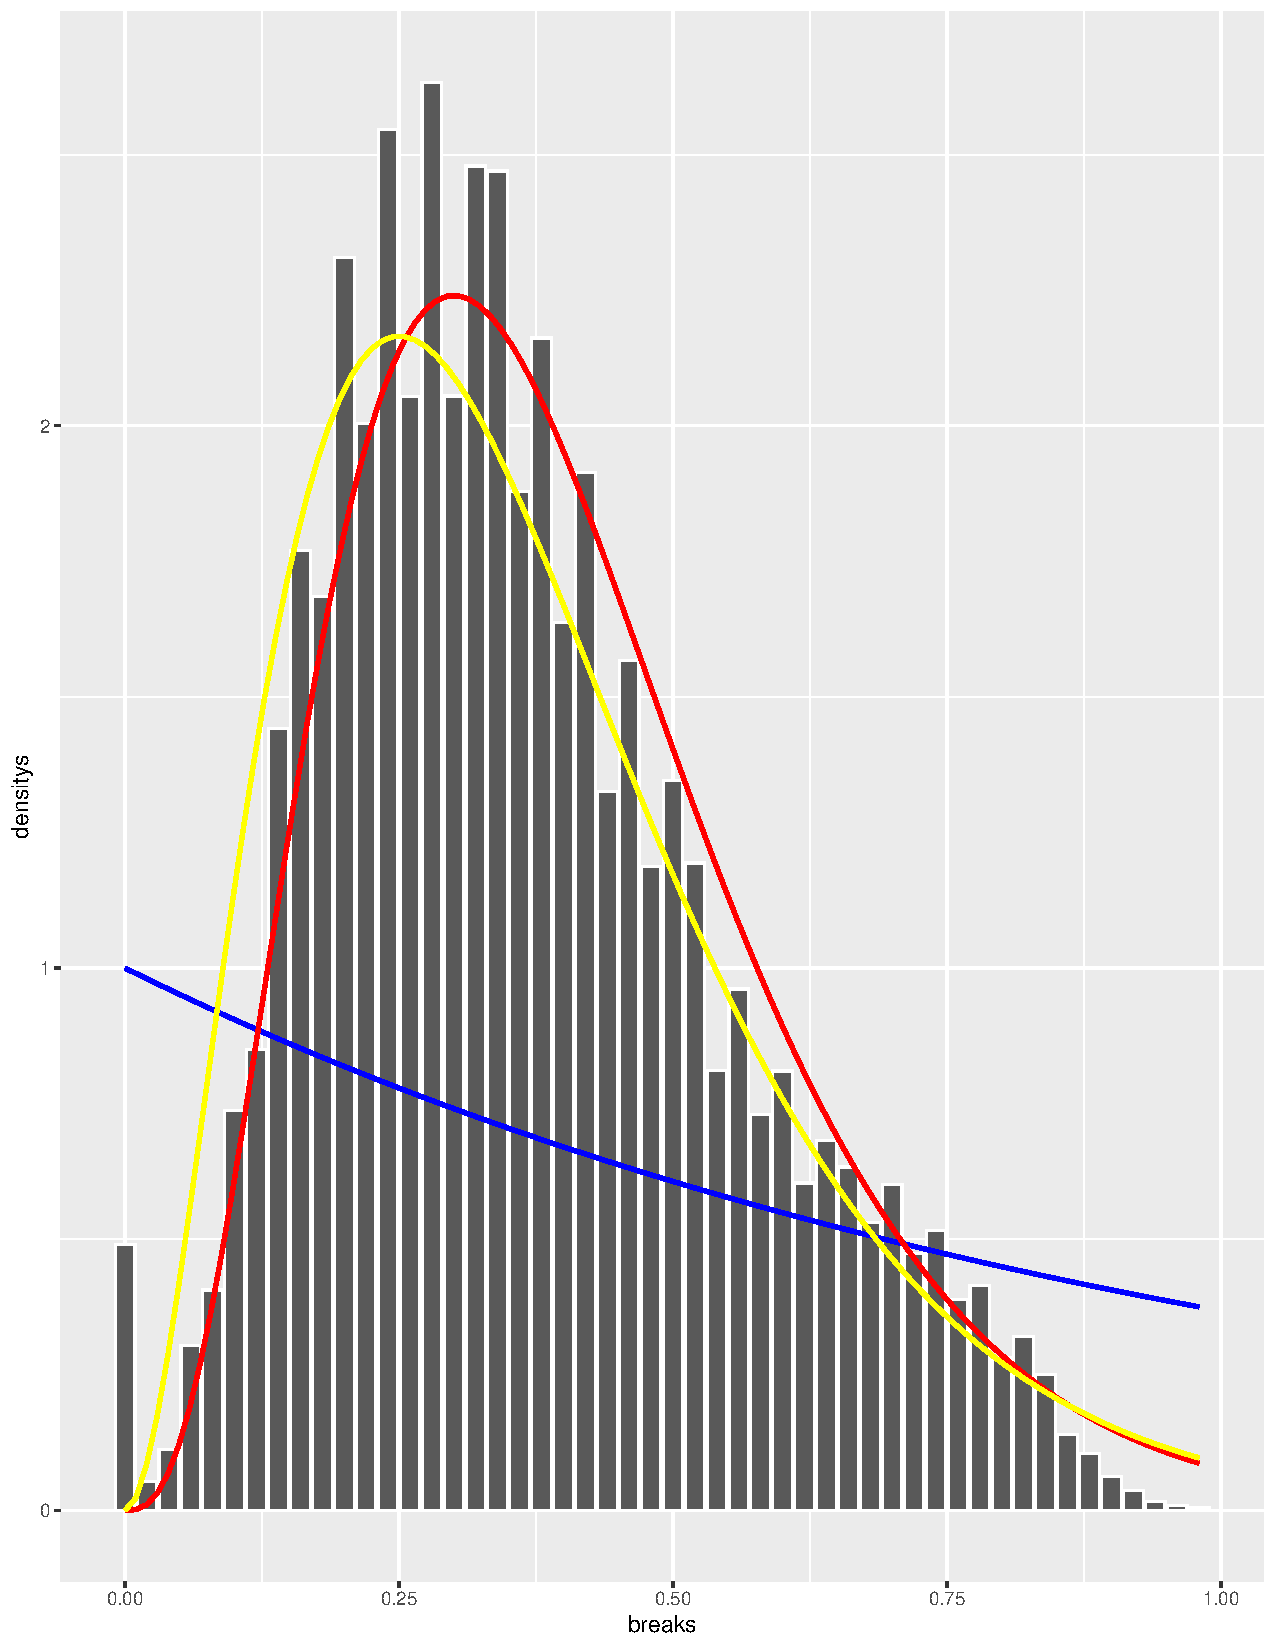
\includegraphics[width=0.7\linewidth,height=0.4\textheight]{Rplot}
	\caption{}
	\label{fig:rplot}
\end{figure}

\noindent The R code :\\
------------------------------------------------------------------------------------------\\
library(png)\\
library(ggplot2)\\
img <- readPNG("/home/jason/Workspace/sar\_home\_work1.png",native =T)\\
img <-abs(img)/(max(abs(img)))\\
a <- hist(img,freq = F,breaks=seq(0,1,0.02),main="Histogram of urban forest")\\
a1 <- a$density$\\
dat <-data.frame(densitys=a1,breaks=seq(0,0.98,0.02))\\
ggplot(dat,aes(x=breaks,y=densitys))+\\
geom\_bar(stat = "identity",colour="white")+\\
stat\_function(fun=dgamma,geom\\ ="line",size=1,col="blue",args=list(shape=1,scale=1))+\\
stat\_function(fun=dgamma,geom\\ ="line",size=1,col="red",args=list(shape=4,scale=1/10))+\\
stat\_function(fun=dgamma,geom\\ ="line",size=1,col="yellow",args=list(shape=3,scale=1/8))\\
------------------------------------------------------------------------------------------\\

\end{document}